\let\negmedspace\undefined
\let\negthickspace\undefined
\documentclass[journal]{IEEEtran}
\usepackage[a5paper, margin=10mm, onecolumn]{geometry}
\usepackage{lmodern} 
\usepackage{tfrupee} 
\setlength{\headheight}{1cm}
\setlength{\headsep}{0mm}   

\usepackage{gvv-book}
\usepackage{gvv}
\usepackage{cite}
\usepackage{amsmath,amssymb,amsfonts,amsthm}
\usepackage{algorithmic}
\usepackage{graphicx}
\usepackage{textcomp}
\usepackage{xcolor}
\usepackage{txfonts}
\usepackage{listings}
\usepackage{enumitem}
\usepackage{mathtools}
\usepackage{gensymb}
\usepackage{comment}
\usepackage[breaklinks=true]{hyperref}
\usepackage{tkz-euclide} 
\usepackage{listings}                             
\def\inputGnumericTable{}                                 
\usepackage[latin1]{inputenc}                                
\usepackage{color}                                            
\usepackage{array}                                            
\usepackage{longtable}                                       
\usepackage{calc}                                             
\usepackage{multirow}                                         
\usepackage{hhline}                                           
\usepackage{ifthen}                                           
\usepackage{lscape}
\usepackage{xparse}

\bibliographystyle{IEEEtran}

\title{4.11.39}
\author{EE25BTECH11062 - Vivek K Kumar}

\begin{document}
\maketitle

\renewcommand{\thefigure}{\theenumi}
\renewcommand{\thetable}{\theenumi}

\numberwithin{equation}{enumi}
\numberwithin{figure}{enumi} 

\textbf{Question}:\\
Find the area of the region bounded by the lines $3x - 2y + 1 = 0$, $2x + 3y - 21 = 0$
and $x - 5y + 9 = 0$

\textbf{Solution: }

\begin{table}[H]    
  \centering
  \begin{tabular}{|c|c|}
\hline
\textbf{Name} & \textbf{Value} \\ \hline
$\vec{A}$ & $\myvec{2 & 1 \\0 & 3}$ \\ \hline
\end{tabular}

  \caption{Variables used}
  \label{tab:4.11.39}
\end{table}

The given lines can be represented as 
\begin{align}
    \vec{n_1}^\top\vec{x} = c_1\\
    \vec{n_2}^\top\vec{x} = c_2\\
    \vec{n_3}^\top\vec{x} = c_3
\end{align}

Let the points of intersections of the given lines be represented as $\vec{A}, \vec{B}, \vec{C}$
\begin{align}
    \myvec{\vec{n_1} & \vec{n_2}}^\top\vec{A} = \myvec{c_1 \\ c_2}\\
    \myvec{\vec{n_2} & \vec{n_3}}^\top\vec{B} = \myvec{c_2 \\ c_3} \\
    \myvec{\vec{n_3} & \vec{n_1}}^\top\vec{C} = \myvec{c_3 \\ c_1} 
\end{align}

The area of the triangle can be then represented as
\begin{align}
    \frac{1}{2} \norm{\vec{A}-\vec{B}}\norm{\vec{C}-\vec{B}} \sqrt{1- \brak{\frac{\vec{n_2}^\top\vec{n_3}}{\norm{\vec{n_2}}\norm{\vec{n_3}}}} ^ 2}
\end{align}

Solving for $\vec{A}, \vec{B}, \vec{C}$
\begin{align}
    \myvec{3 & -2 \\ 2 & 3}\vec{A} = \myvec{-1 \\ 21} \\ 
   \implies \myaugvec{2}{3 & -2 & -1 \\ 2 & 3 & 21} \xleftrightarrow[]{R_2 \leftarrow R_2-2/3R_1} \myaugvec{2}{3 & -2 & -1 \\ 0 & 13/3 & 65/3}\\
   \vec{A} = \myvec{3 \\ 5}\\
    \myvec{2 & 3 \\ 1 & -5}\vec{B} = \myvec{21 \\ -9} \\ 
    \implies \myaugvec{2}{2 & 3 & 21 \\ 1 & -5 & -9} \xleftrightarrow[]{R_2 \leftarrow R_2-1/2R_1} \myaugvec{2}{2 & 3 & 21 \\ 0 & -13/2 & -39/2}\\
   \vec{B} = \myvec{6 \\ 3}\\
    \myvec{1 & -5 \\ 3 & -2}\vec{C} = \myvec{-9 \\ -1} \\ 
    \implies \myaugvec{2}{1 & -5 & -9 \\ 3 & -2 & -1} \xleftrightarrow[]{R_2 \leftarrow R_2-3R_1} \myaugvec{2}{1 & -5 & -9 \\ 0 & 13 & 26}\\
   \vec{C} = \myvec{1 \\ 2}
\end{align}
Area of the triangle from the above equations is
\begin{align}
    \frac{1}{2}\norm{\myvec{-3 & 2}^\top}\norm{\myvec{-5 & -1}^\top}\sqrt{1 - \brak{\frac{-13}{13\sqrt{2}}}^2} = \frac{13}{2}
\end{align}

\begin{figure}[H]
   \centering
  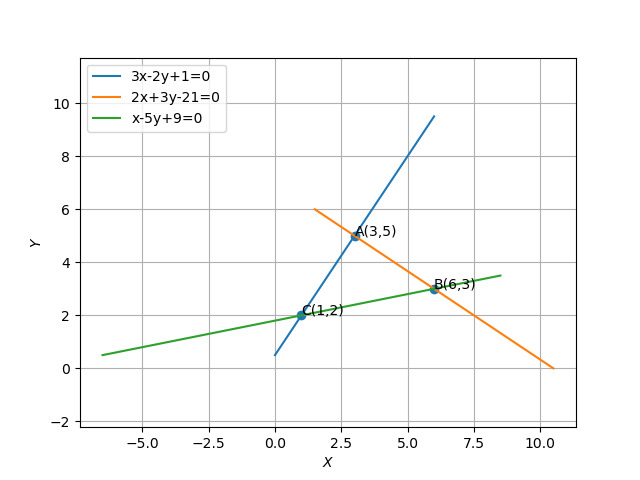
\includegraphics[width=0.64\columnwidth]{figs/fig.png}
   \caption{Triangle enclosed by given lines}
   \label{stemplot}
\end{figure}
\end{document}  